\documentclass{article}
\usepackage{pgfplots}
\usepackage{graphicx}
\begin{document}
  \title{Using Circles to Approximate Riemann Sums}
  \author{Evan Derby}
  \date{11 December 2015}
  \maketitle

  \section{Introduction}
    Riemann Sums are a method of approximating the area underneath a curve by
    adding up the areas of shapes, usually rectangles, whose height is bound by
    a point on the function. As the width of these shapes approaches zero, the
    summation approaches the Riemann integral, the true area underneath the
    curve.

    \[ \displaystyle\lim_{n \to \infty}\sum_{i=1}^{n} f(x^*_i) \left(\frac{b-a}{n}\right) = \int\limits_a^b f(x)dx \]

    Riemann sums can be approximated three different ways, all of which depend on
    where the rectangle intercepts the curve. When the rectangle's top right
    vertex is bounded by the curve, this is known as a RRAM, or Right-hand
    Rectangular Approximation Method. The same goes for a left-bounded rectangle
     (LRAM), and a rectangle whose midpoint intercepts the curve (MRAM). The
    formula changes slightly for each method, denoted by \( x^*_i \). For LRAM,
    \( x_i^* = x_{i-1} \); RRAM, \( x_i^* = x_i \); and MRAM, \( x_i^* = \frac{1}{2}(x_i + x_{i-1}) \).

    \begin{figure}[h]
      \centering
      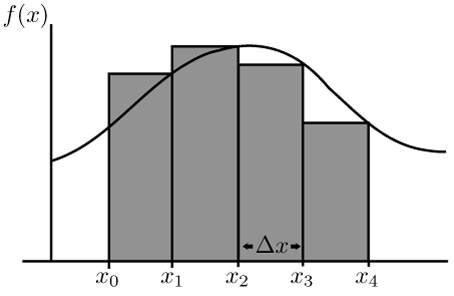
\includegraphics[width=0.5\textwidth]{riemann_1}
      \caption{A function with Right-hand Riemann sum rectangles drawn underneath.}
    \end{figure}

    Riemann sums are not limited to rectangles, however. Another, more accurate method of
    approximation makes use of trapezoids, whose area formula is comparably
    simple to that of a rectangle's. Trapezoidal approximation is similar to
    the result of averaging a left and right approximation. This method makes
    use of the trapezoid area formula \( A = \frac{1}{2}h(b_1+b_2) \). A Riemann
    sum constructed with trapezoids takes this form:

    \[ \displaystyle\lim_{n \to \infty}\frac{1}{2}\Delta x\sum_{i=1}^n f(a+i\Delta x) \]

    Historically, Riemann's definition was the first rigourous definition of the
    integral of a function on an interval. Thus, in Calculus classes today, it is often
    the first introduction students recieve to the idea of calculating the area
    under a curve; the AP Calculus Syllabus even specifies Riemann sums as the
    first material in the Integrals unit.\footnote{http://media.collegeboard.com/digitalServices/pdf/ap/ap-calculus-course-description.pdf}

    As a student who was introduced to integration with Riemann sums, I often
    wondered: are there other shapes that you could use or approximations similar
    to Riemann's that would behave similarly? In this paper I intend to
    investigate just that: are circles a viable shape to use in the fashion of
    a Riemann sum? How accurate is such an approximation? Does this approximation
    behave like a Riemann sum in that its limit approaches the real area under
    the curve?

    In this investigation, I'll derive this approximation (hereafter called the
     Circle sum) in a similar method to how Riemann sums can be derived.
    I'll then test each of my questions. I'll compare the efficacy of a Circle
    sum versus a similar Riemann sum, as well as examine the behavior of the Circle
    sum as it approaches infinity.

  \section{Derivation}
    The Riemann sum can be simply derived by finding the area of a rectangle under
    the curve, summing all such rectangles between two bounds, and finally taking
    the limit of this summation as the number of rectangles approaches infinity.
    In order to find a Circle sum, a similar process will be followed.

    \subsection{Riemann}
    We begin by being given a function \( f(x) \) and a set of bounds \( a \) and
    \( b \). The width of the workable area is defined as \( b-a \). Thus, we can
    divide the workable area into \( n \) partitions, each with a width of \( \Delta x = \frac{b-a}{n} \).
    The right-bound x-value for any such rectangle inside of these bounds can be
    found by adding the partition width \( n \) times for the \(n\)th partition.
    Such a rectangle on the curve has width \( \Delta x \) and height
    \( f(a+n_i\Delta x) \). Thus, the area of this rectangle is \( f(a+n_i\Delta x)\Delta x \).
    This rectangle would appear below the function in this manner:

    The sum of the rectangles that exist from \( a \) to \( b \) can be expressed
    with summation notation:

    \[ A_{total} = f(a+(0)\Delta x)\Delta x + f(a+(1)\Delta x)\Delta x + \dots + f(a+n\Delta x)\Delta x \]

    \[ = \displaystyle\sum_{i=0}^n f(a+i\Delta x)\Delta x \]

    \( A_{total} \) is represented by the shaded green areas in Figure 3.

    When we take the limit of \( A_{total} \) as the number of partitions, \( n \),
    approaches infinity, we find that \( A_{total} \) approaches \( A_{real} \),
    given by integrating the function from \( a \) to \( b \).

    \[ \displaystyle\lim_{n \to \infty}\sum_{i=0}^n f(a+i\Delta x)\Delta x = \int\limits_a^b f(x)dx \]


\end{document}
